%% Template baseado no do Prof. Arnaldo Mandel
%% Veja https://www.ime.usp.br/~am/414/listas/index.html

\documentclass[12pt]{article}

%% Escrevendo em português:

%\usepackage[brazilian]{babel}
\usepackage[utf8]{inputenc}
\usepackage[T1]{fontenc}
\usepackage{textcomp}
\usepackage[T1]{fontenc}
%----------------------------

\setlength{\topmargin}{-.5in}
\setlength{\textheight}{9in}
\setlength{\textwidth}{6.3in}
\setlength{\oddsidemargin}{-.125in}
\setlength{\evensidemargin}{-.125in}

\usepackage[usestackEOL]{stackengine}
\usepackage{xspace}
\usepackage{pifont}
\usepackage{amsmath}
\usepackage{amsfonts}
\usepackage[dvipsnames]{xcolor}
\usepackage{fancybox}
\usepackage{amsthm}
\usepackage{listings}
\usepackage{hyperref}
\usepackage{todonotes}

\usepackage{MnSymbol,wasysym}
\usepackage{marvosym}

\pagestyle{empty}

\definecolor{darkgreen}{RGB}{0, 133, 117}
\definecolor{yelloworange}{HTML}{FAA21A}

\newcommand{\N}{{\tt I\kern-.2em N \relax}}      % N        |N
\def\pule{\vspace{0.2cm}}
\def\pulao{\vspace{0.5cm}}
\def\pulaozao{\vspace{1cm}}
\def\ni{\noindent}

\newcommand{\Si}{\ensuremath{\Sigma}\xspace}
\newcommand{\Sis}{\ensuremath{\Sigma^*}\xspace}
\newcommand{\Ga}{\ensuremath{\Gamma}\xspace}
\newcommand{\Gas}{\ensuremath{\Gamma^*}\xspace}
\newcommand{\serio}{\ding{98}\xspace}
\newcommand{\LP}{L\&P\xspace}
\newcommand{\conj}[2]{\ensuremath{\{#1\,|\;#2\}}}
\DeclareMathOperator{\Ima}{Im}
\newcommand{\ssq}{\ensuremath{\subseteq}\xspace}
\newcommand{\union}{\mathop{\bigcup}\displaylimits}
\newcommand{\Rfield}[1]{\ensuremath{\mathbb{R}^{#1}}\xspace}
\newcommand{\del}{\ensuremath{\text{d}}\xspace}
\newcommand{\expct}[1]{\ensuremath{\langle {#1} \rangle}\xspace}

\begin{document}

\newtheorem{theorem}{Teorema}%[section]
\newtheorem{corollary}{Corolário}[theorem]
\newtheorem{lemma}[theorem]{Lema}

\begin{center}
\Huge \bf
Parallelizing GCC with Threads
\vspace{0.5cm}
\end{center}
\tiny{\ }
\begin{figure}[ht]
     \centering
     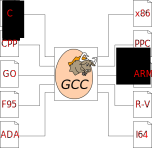
\includegraphics[scale=1.]{logo.pdf}
     \label{fig:logo}
\end{figure}
\vspace*{\fill} \\
\normalsize{
\textcolor{darkgreen}{Giuliano Belinassi} \\
University of São Paulo -- Brazil \\
IRC: giulianob \\
Email: \href{mailto:giuliano.belinassi@usp.br}{\texttt{giuliano.belinassi@usp.br}} \\
Github: \url{https://github.com/giulianobelinassi/} \\
Date: \today
}
\newpage

\begin{section}{About Me}
    Currently pursuing a Master's Degree in Computer Science at the University
    of São Paulo with a Computer Science Bachelor's degree in the same
    institution. I've always been fascinated by topics such as
    High-Performance Computing and Code Optimization, and I am currently
    researching topics in compiler
    parallelization. Therefore, I am applying to the GNU Compiler Collections
    (GCC) both as a research project in parallelization of compilers, and
    mainly to become a part of the free software community.

    \textbf{Skills}: Strong knowledge in C, Vim, and command line utilities (grep, sed, ...)
\end{section}

\begin{subsection}{Contributions to GCC}

I've submitted some patches, mainly adding inline optimizations to
trigonometric functions. These patches required deep testing to guarantee
that the optimization did not yield severely incorrect results, which
concluded in a blogpost about the patch \textit{Optimize $\sin (\arctan (x))$}.
I did this blogpost both to register how to add these new kinds of optimizations,
and also to encourage newcomers to contribute to GCC.

\begin{table}[!htbp]
\centering
\begin{tabular}{|l|l|}
\hline
Name                                                                                      & Status   \\ \hline
    \href{https://patchwork.ozlabs.org/patch/981596/}{Optimize $\sin (\arctan (x))$}      & \color{darkgreen}{\texttt{Accepted}} \\ \hline
    \href{https://patchwork.ozlabs.org/patch/1003988/}{Optimize $\sinh (\text{arctanh} (x))$}   & \color{darkgreen}{\texttt{Accepted}} \\ \hline
    \href{https://patchwork.ozlabs.org/patch/961362/}{Fix typo 'exapnded'}                & \color{darkgreen}{\texttt{Accepted}} \\ \hline
    \href{https://en.wikibooks.org/wiki/LaTeX/Hyperlinks}{Split 'opt and gen' variable}   & \color{yelloworange}{\texttt{Working}} \\ \hline
    \href{https://patchwork.ozlabs.org/patch/1023211/}{Update $\sin (\arctan (x))$ test}  & \color{yelloworange}{\texttt{Waiting Stage1}} \\ \hline
    \href{https://patchwork.ozlabs.org/patch/1046302/}{Fix PR89437}                           & Wilco Dijkstra version accepted \\ \hline
\end{tabular}
\end{table}

\end{subsection}

\begin{section}{Paralelization Project}

Even before Google released the list of GSoC accepted organizations, I started
discussing this project in the mailing
list\footnote{\url{https://gcc.gnu.org/ml/gcc/2018-11/msg00073.html}}. Having worked
with parallelism before and having an interest in working with compilers, I got
interested in this project.

As stated in PR84402\footnote{\url{https://gcc.gnu.org/bugzilla/show\_bug.cgi?id=84402}},
there is a parallelism bottleneck in GCC concerning huge files, with hundreds of
thousends of lines of code. Further discussion in the mailing list made
Bin Cheng\footnote{\url{https://gcc.gnu.org/ml/gcc/2018-12/msg00079.html}} report that
he is facing a similar issue with his project, stating that parallelizing the
compiler may solve his problem. These topics supports the interest in the
community for this project.

\end{section}

\begin{subsection}{Current Status}
I already developed a way to measure the effectiveness of the parallel implementation.
First, I developed a tool to collect and analyze the compilation time of GCC, with
support to the GCC bootstrap, and a script to plot the timing data; as available
in \footnote{\url{https://github.com/giulianobelinassi/gcc-timer-analysis}}.
I have access to a 64 cores Opteron machine to run the tests, and I managed to
    reproduce the PR84402 bottleneck in it, as illustrated in Figure \ref{fig:analysis}.
I am also using the generated \texttt{gimple-match.c} file in order to measure the elapsed
time of a single file.


I also explored the GCC codebase in order to find the performance bottleneck for
such huge files. Analyzing the most time-consuming file in GCC's project
(\texttt{gimple-match.c}), I found that the method
\texttt{finalize\_compilation\_unit} of
class \texttt{symbol\_table} takes around 50s to compile with a
\texttt{--disable-checking} GCC under \texttt{-O2}, with the \texttt{expand\_all\_functions}
routine taking most of this time. Currently, my strategy is to try to parallelize
this part of the compilation, as it seems possible because I've already made GCC output
functions in reverse orders.

Furthermore, I am also studying the theoretical background behind \texttt{GIMPLE},
and \texttt{cgraphs}. I have read the GIMPLE
documentation\footnote{\url{https://gcc.gnu.org/onlinedocs/gccint/}}, and
I am looking for how \texttt{cgraph} works internally, both in theory and in
GCC.

\end{subsection}

\begin{subsection}{Planned Tasks}
    Currently, my plan consists in three high-level topics, but more details
will be provided as I proceed into the project. These topics are:

\begin{enumerate}
    \item \textit{Document the global variables and states}. The \texttt{cgraph}
clearly was not implemented with this kind of parallelism in mind, as it has a lot
of global states (i. e., RTL initialization, possible node dependency,
Garbage Collector, ...). This has to be transformed into something that could
be handled locally, or insert locks.
	\item \textit{Develop a parallel prototype}. GCC supports a lot of systems
with different threading schemes. Discussion in the mailing list suggested the
use of pthreads and C++11 threads, however, this may not be the easiest way to
develop parallel software.
	\item \textit{Refactor the parallel prototype}. Here the aim is to improve
the previous implementation with proper cross-platform support.
\end{enumerate}


\begin{figure}[ht]
 \centering
 \includegraphics[scale=0.6, angle=-90]{out-crop.pdf}
 \caption{Elapsed time analysis in GCC compilation for a 64 cores machine, No bootstrap}
 \label{fig:analysis}
\end{figure}

\end{subsection}

\end{document}
